\documentclass[aspectratio=169,11pt]{beamer}
\usepackage[utf8]{inputenc}
\usepackage[T1]{fontenc}
\usepackage[spanish]{babel}
\usepackage{amsmath,amssymb}
\usepackage{tikz}
\usetikzlibrary{arrows.meta,angles,calc,positioning}
\usetheme{Madrid}
\usecolortheme{default}
\setbeamertemplate{navigation symbols}{}
\setbeamertemplate{blocks}[rounded][shadow=false]
\newcommand{\ang}[1]{\angle #1^\circ}

\title[Incertidumbre y templates]{Paso 7: Incertidumbre y templates}
\subtitle{Una planta que no se conoce: una nube de puntos en cada frecuencia}
\author{Curso de control robusto (QFT)}
\date{}
\begin{document}
\begin{frame}\titlepage\end{frame}

\begin{frame}{Dónde encaja este paso}
  \tiny
  \begin{enumerate}\setlength{\itemsep}{-2pt}
    \item[1.] Números complejos \hfill \textcolor{gray}{(hecho)}
    \item[2.] Funciones de transferencia: $s$, polos y ceros \hfill \textcolor{gray}{(hecho)}
    \item[3.] Respuesta en frecuencia: $s=j\omega$, magnitud y fase \hfill \textcolor{gray}{(hecho)}
    \item[4.] Decibelios y escala logarítmica (Bode) \hfill \textcolor{gray}{(hecho)}
    \item[5.] Realimentación: $L$, $T=\frac{L}{1+L}$, $S=\frac{1}{1+L}$ \hfill \textcolor{gray}{(hecho)}
    \item[6.] Nichols chart \hfill \textcolor{gray}{(hecho)}
    \item[\textbf{7.}] \textbf{Incertidumbre y templates} \hfill $\leftarrow$ estamos aquí
    \item[8.] Especificaciones $\rightarrow$ bounds
    \item[9.] Loop shaping, prefiltro y verificación
    \item[10.] QFT en control digital
    \item[11.] Dos caminos digitales: $z$ y $w$
    \item[12.] Estabilidad, límites, más especificaciones y caso real
    \item[13.] Muestreo por eventos con periodo base $T$
    \item[14.] Sistemas de dos estados: lazo interno y externo
    \item[15.] QFT y sistemas no lineales
    \item[16.] Algoritmos de QFT: cómo funcionan por dentro
    \item[17.] QFT en Python: una biblioteca paso a paso
    \item[18.] QFT en MATLAB: el mismo código, otra sintaxis
    \item[19.] Historia, panorama y bibliografía
  \end{enumerate}
  \vspace{2pt}
  \begin{block}{Objetivo de hoy}
    Pasar de ``una planta'' a ``una familia de plantas'' y ver qué aspecto tiene en el Nichols: el \textbf{template}.
  \end{block}
\end{frame}

\begin{frame}{Por qué incertidumbre}
  \small
  \begin{itemize}
    \item $P(s)$ es un \textbf{modelo}: la planta real cambia con la carga, el desgaste, la temperatura, la unidad que te toque.
    \item Un diseño hecho para un único $P$ puede dejar de funcionar si los parámetros se mueven.
    \item QFT trabaja con un \textbf{conjunto} de plantas $\mathcal{P}=\{P_1,P_2,\dots\}$ y exige que \emph{todas} cumplan las especificaciones.
  \end{itemize}
  \begin{block}{Ejemplo que usaremos hasta el paso 9}
    \[ P(s)=\frac{K}{s\,(s+a)},\qquad K\in[1,5],\quad a\in[1,3] \]
    Un motor con integrador: $K$ es la ganancia (varía de 1 a 5, es decir, $14$ dB) y $a$ el polo mecánico (de 1 a 3). Cada pareja $(K,a)$ es una planta posible. \textbf{Nominal}: $P_0$ con $K=1$, $a=1$.
  \end{block}
\end{frame}

\begin{frame}{La familia en un Bode}
  \footnotesize
  \begin{columns}[T]
  \begin{column}{0.62\textwidth}
    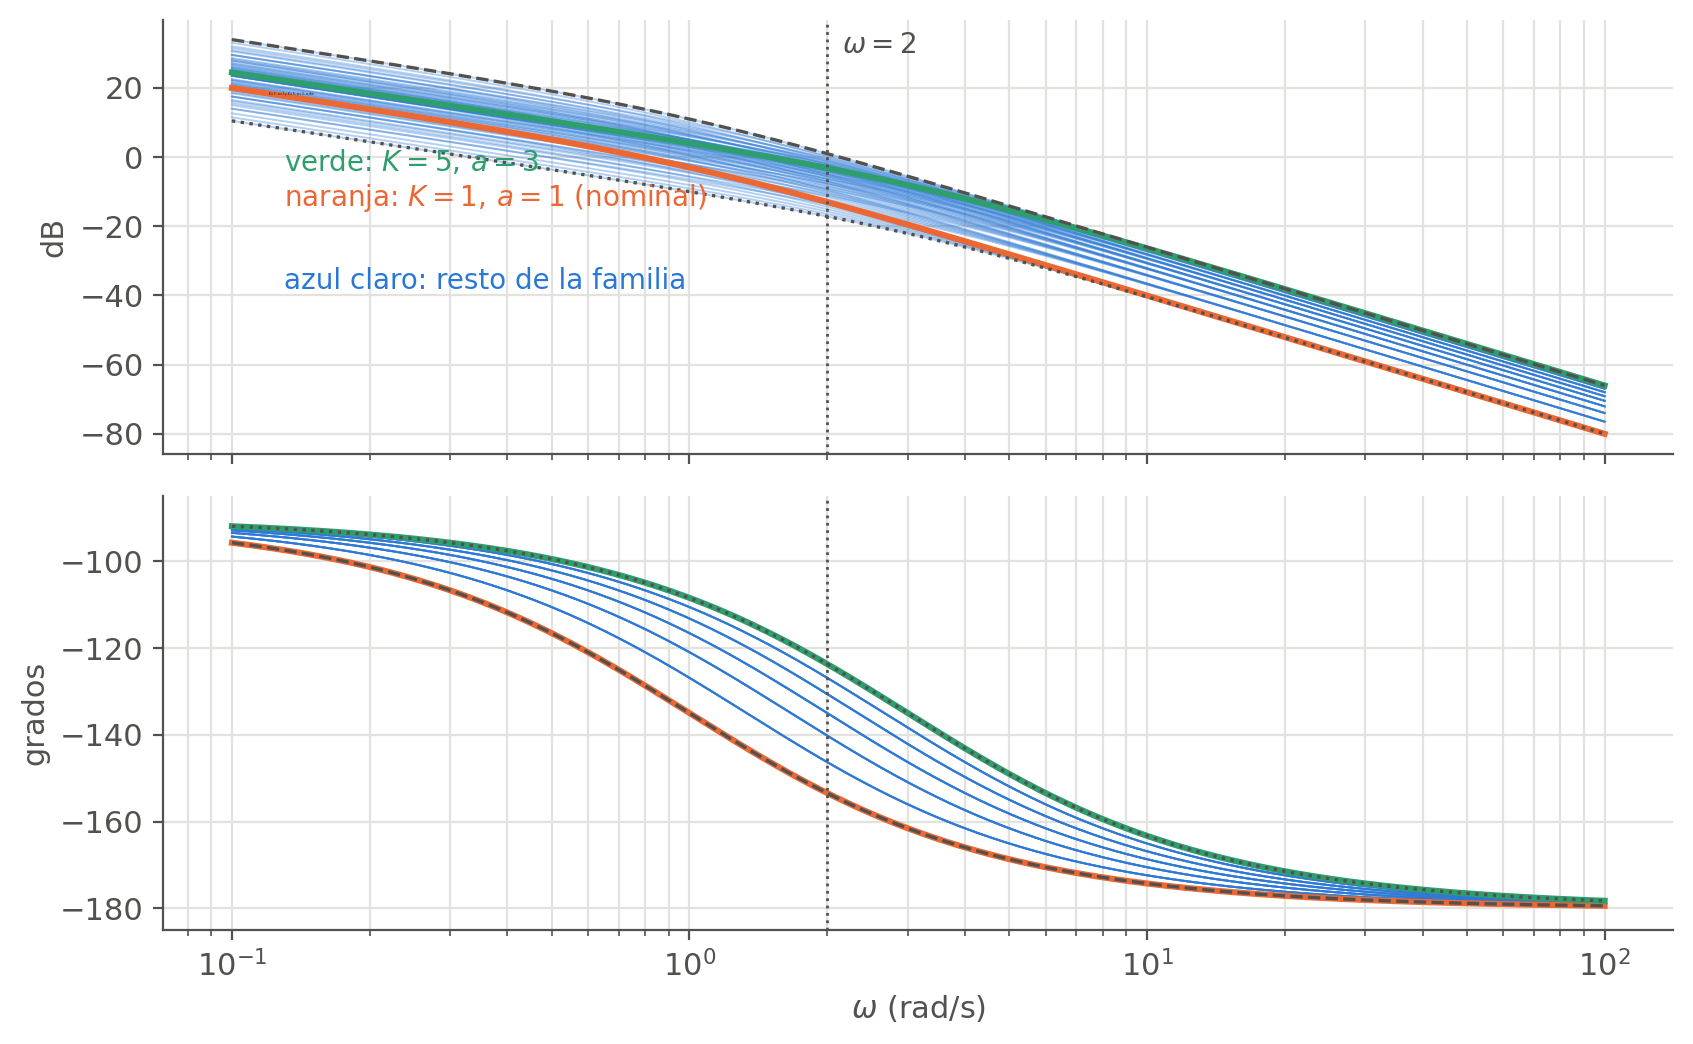
\includegraphics[width=\textwidth]{fig/familia_bode.png}
  \end{column}
  \begin{column}{0.36\textwidth}
    \begin{itemize}
      \item Cada $(K,a)$ da una curva; todas juntas forman una \textbf{banda}.
      \item En cada $\omega$ la banda tiene un ancho en dB y otro en grados.
      \item A bajas $\omega$ domina $K/a$; a altas, $K/\omega^2$.
    \end{itemize}
    \begin{block}{Lo que importa}
      La banda en una $\omega$ fija es lo que luego pasaremos al Nichols.
    \end{block}
  \end{column}
  \end{columns}
\end{frame}

\begin{frame}{En una frecuencia: cada planta es un punto del mapa}
  \footnotesize
  \begin{columns}[T]
  \begin{column}{0.58\textwidth}
    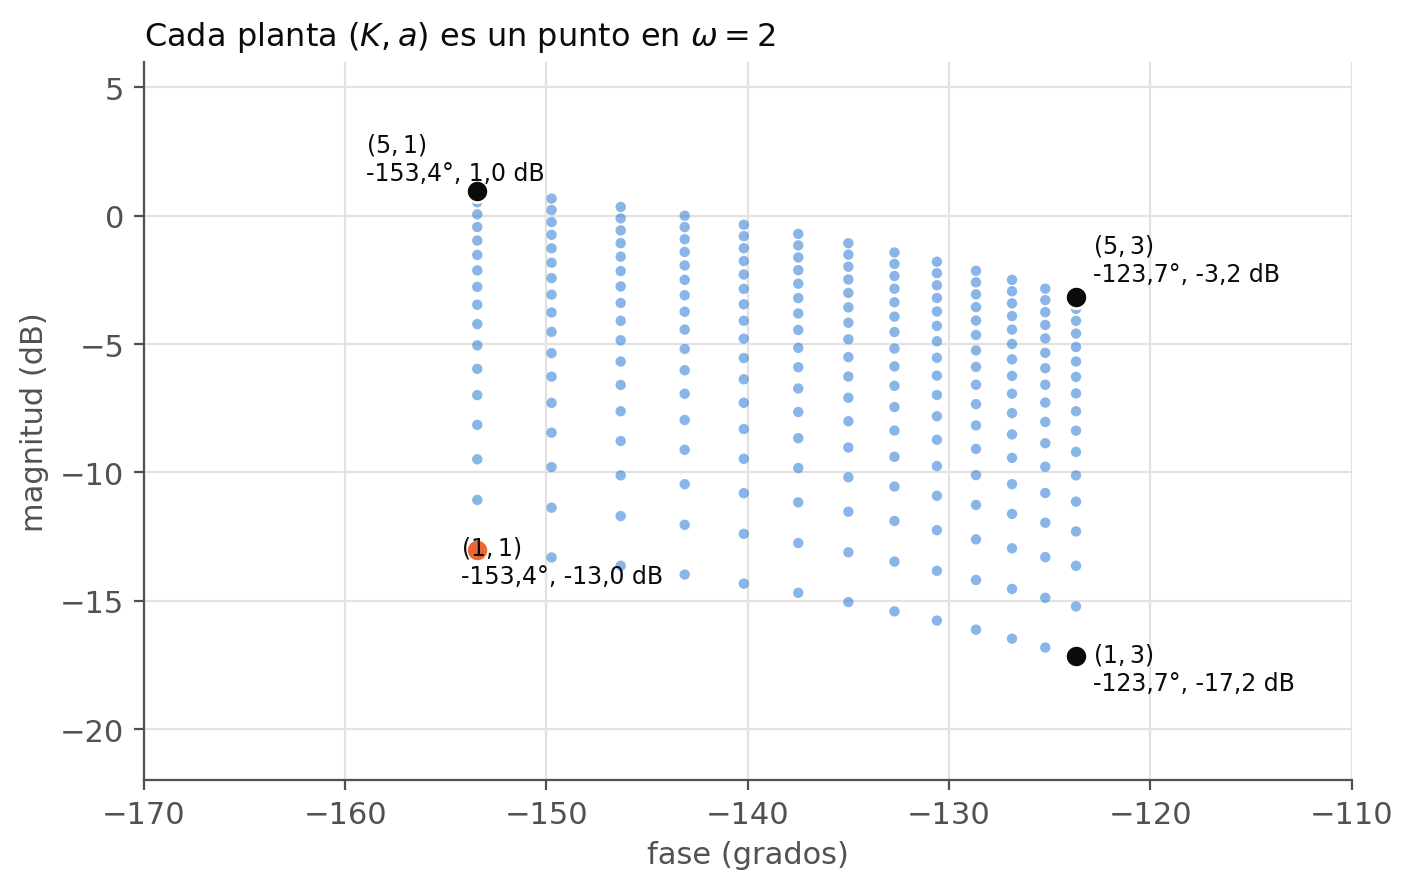
\includegraphics[width=\textwidth]{fig/nube_w2.png}
  \end{column}
  \begin{column}{0.4\textwidth}
    Fijamos $\omega=2$. Cada planta $(K,a)$ da un número complejo $P(j2)$, es decir, un punto $(\angle P,\ |P|_{\text{dB}})$ (paso 6).
    \begin{block}{Las cuatro esquinas}
      \begin{tabular}{c|c|c}
        $(K,a)$ & fase & dB\\\hline
        (1,1) & $-153.4^\circ$ & $-13.0$\\
        (1,3) & $-123.7^\circ$ & $-17.2$\\
        (5,1) & $-153.4^\circ$ & $+1.0$\\
        (5,3) & $-123.7^\circ$ & $-3.2$
      \end{tabular}
    \end{block}
    La nube ocupa una región de unos $30^\circ$ de ancho y $18$ dB de alto.
  \end{column}
  \end{columns}
\end{frame}

\begin{frame}{Definición: el template}
  \small
  \begin{block}{Template en la frecuencia $\omega_i$}
    $\mathcal{T}(\omega_i)=\{\,P(j\omega_i)\ :\ P\in\mathcal{P}\,\}$ dibujado en el mapa de Nichols.
  \end{block}
  \begin{itemize}
    \item Es la \textbf{región} que ocupan todas las plantas posibles, en esa frecuencia concreta.
    \item Hay un template por frecuencia: cambia de forma, tamaño y posición con $\omega$.
    \item Cuanto más ancho el template, más incertidumbre hay que absorber con el controlador.
  \end{itemize}
  \begin{alertblock}{Cómo se construye en la práctica}
    \begin{enumerate}
      \item Tomar una malla de parámetros $(K,a)$ que cubra el rango (incluye los bordes).
      \item Para cada una, calcular $P(j\omega_i)$ y pasarlo a (fase, dB).
      \item Dibujar la región cerrada que contiene todos los puntos (basta el contorno).
    \end{enumerate}
  \end{alertblock}
\end{frame}

\begin{frame}{Los templates cambian con la frecuencia}
  \footnotesize
  \begin{columns}[T]
  \begin{column}{0.64\textwidth}
    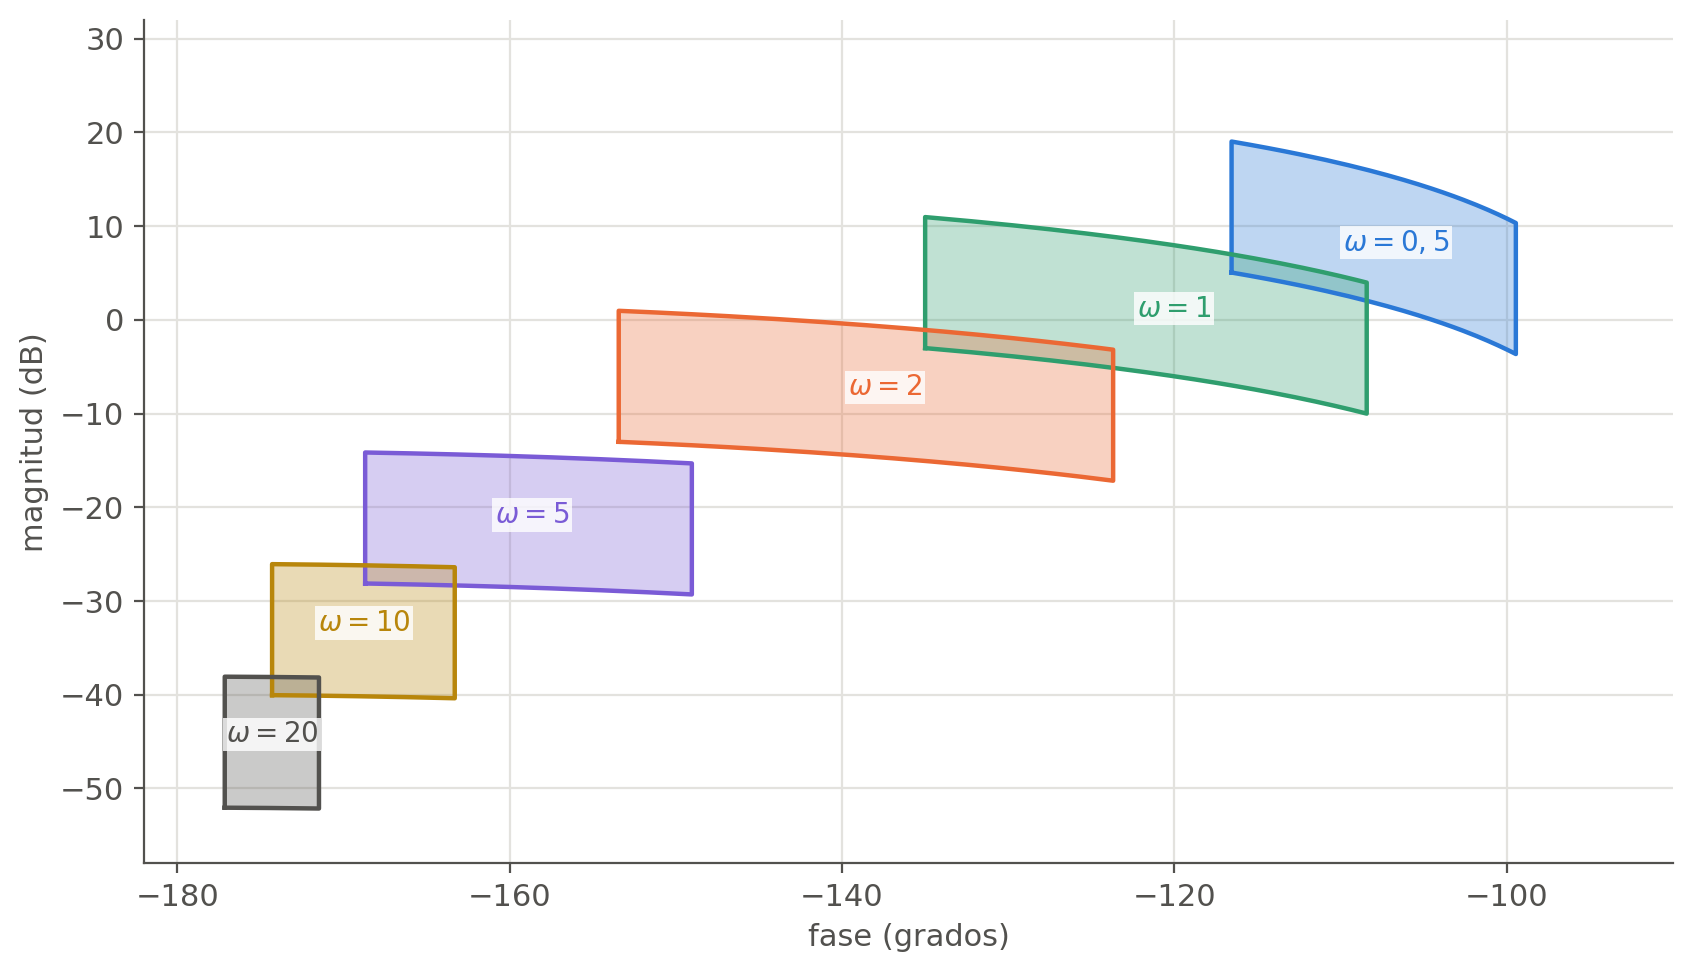
\includegraphics[width=\textwidth]{fig/templates.png}
  \end{column}
  \begin{column}{0.34\textwidth}
    \begin{itemize}
      \item $\omega$ baja: fase cerca de $-90^\circ$, templates \textbf{altos} (mucha variación de ganancia).
      \item $\omega$ alta: fase cerca de $-180^\circ$, templates \textbf{pequeños} y abajo (la ganancia varía solo por $K$).
      \item Barrer $\omega$ de menor a mayor lleva el template hacia abajo y a la izquierda.
    \end{itemize}
    \begin{block}{Idea clave}
      El template depende solo de la \textbf{planta} y de $\omega$, no del controlador.
    \end{block}
  \end{column}
  \end{columns}
\end{frame}

\begin{frame}{El controlador traslada el template sin deformarlo}
  \footnotesize
  \begin{columns}[T]
  \begin{column}{0.58\textwidth}
    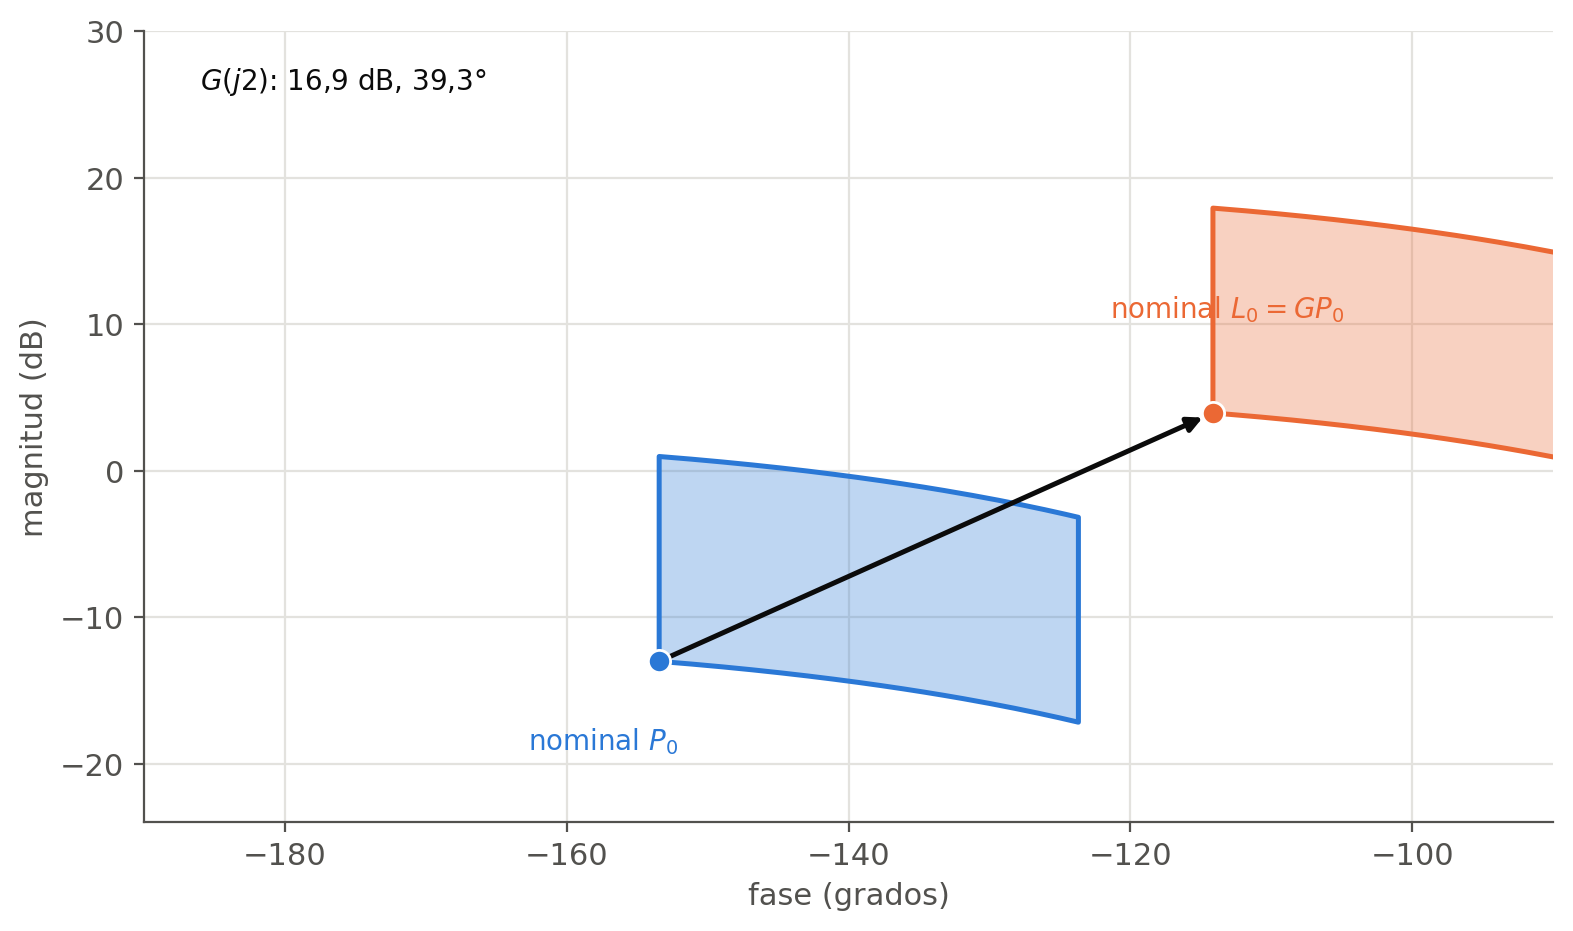
\includegraphics[width=\textwidth]{fig/traslacion.png}
  \end{column}
  \begin{column}{0.4\textwidth}
    En $\omega=2$ el controlador $G$ vale $G(j2)=7.04\angle39.3^\circ$ ($16.9$ dB, $39.3^\circ$). Cada planta $P_i$ pasa a ser $L_i=G\,P_i$:
    \[ |L_i|_{\text{dB}}=|G|_{\text{dB}}+|P_i|_{\text{dB}},\quad \angle L_i=\angle G+\angle P_i \]
    Todos los puntos reciben \textbf{el mismo vector} $(+39.3^\circ,\ +16.9\text{ dB})$: el template se desplaza entero.
    \begin{block}{Por qué es útil}
      Basta seguir \textbf{un punto}, el nominal $L_0=GP_0$: donde esté él, está todo el template.
    \end{block}
  \end{column}
  \end{columns}
\end{frame}

\begin{frame}{Qué viene a continuación}
  \small
  \begin{block}{Paso 8: de la especificación al bound}
    Para cada $\omega_i$, ``deslizamos'' el template por el mapa y marcamos en qué posiciones del nominal \emph{todas} las plantas cumplen la especificación. El borde de esa zona es el \textbf{bound}.
  \end{block}
  \begin{block}{Paso 9: loop shaping}
    Elegir $G$ para que $L_0(j\omega_i)$ quede del lado bueno de cada bound.
  \end{block}
  \begin{alertblock}{Por qué funciona}
    Un único punto (el nominal) representa a toda la familia. La incertidumbre se ha convertido en una forma fija, el template, que solo se traslada.
  \end{alertblock}
\end{frame}

\begin{frame}{Ejercicio}
  \small
  Con la planta $P(s)=\dfrac{K}{s(s+a)}$ y $\omega=2$:
  \begin{enumerate}
    \item Calcula $|P(j2)|$ en dB y $\angle P(j2)$ para $(K,a)=(1,1)$ y $(5,3)$.
    \item Con esos dos puntos, ¿qué anchura tiene el template en fase y en dB?
    \item Si $G(j2)=7.04\angle39.3^\circ$, ¿dónde queda el nominal $L_0=GP_0$?
  \end{enumerate}
  \begin{block}{Pista}
    $|P(j\omega)|=\dfrac{K}{\omega\sqrt{\omega^2+a^2}}$ y $\angle P=-90^\circ-\arctan(\omega/a)$.
  \end{block}
  \textcolor{gray}{Solución en el apéndice.}
\end{frame}

\begin{frame}{Resumen}
  \small
  \begin{itemize}
    \item Incertidumbre = una familia de plantas $\mathcal{P}$; cada una es un punto en cada frecuencia.
    \item \textbf{Template} = región de (fase, dB) que ocupan todas las plantas en una $\omega$ dada.
    \item Cambia con $\omega$ (grandes y altos a baja frecuencia, pequeños a alta).
    \item Multiplicar por $G(j\omega)$ \textbf{traslada} el template; no lo deforma.
    \item Por eso se puede diseñar mirando un solo punto, el nominal.
  \end{itemize}
\end{frame}

\appendix
\begin{frame}\centering\Large Apéndice\end{frame}

\begin{frame}{Solución del ejercicio}
  \footnotesize
  \begin{columns}[T]
  \begin{column}{0.54\textwidth}
    \textbf{1.} $\omega=2$:\\
    $(1,1)$: $|P|=\dfrac{1}{2\sqrt{5}}=0.2236\Rightarrow-13.01$ dB; $\angle P=-90^\circ-63.43^\circ=-153.43^\circ$.\\[2pt]
    $(5,3)$: $|P|=\dfrac{5}{2\sqrt{13}}=0.693\Rightarrow-3.18$ dB; $\angle P=-90^\circ-33.69^\circ=-123.69^\circ$.\\[3pt]
    \textbf{2.} Esquinas: $(1,1)$ da el mínimo de dB y la fase más baja; $(5,3)$ la fase más alta. Fase: $-153.4^\circ$ a $-123.7^\circ$, anchura $29.7^\circ$. dB: de $-17.2$ ($(1,3)$) a $+1.0$ ($(5,1)$), anchura $18.2$ dB.\\[3pt]
    \textbf{3.} $L_0=GP_0$: $-13.01+16.95=3.94$ dB y $-153.43^\circ+39.29^\circ=-114.1^\circ$.
  \end{column}
  \begin{column}{0.44\textwidth}
    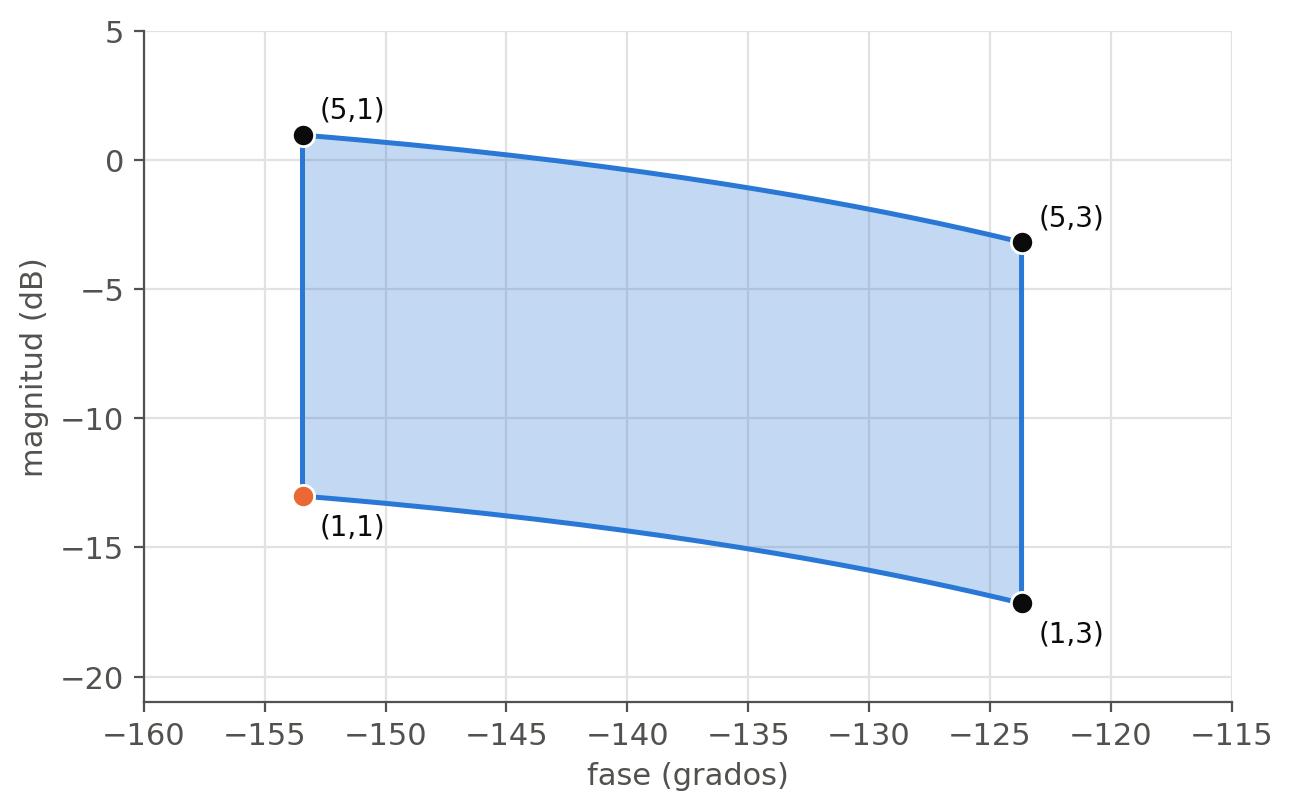
\includegraphics[width=\textwidth]{fig/solucion.png}
  \end{column}
  \end{columns}
\end{frame}

\begin{frame}{Para curiosos: ¿basta con los bordes de la caja de parámetros?}
  \small
  En este ejemplo la fase solo depende de $a$ y el módulo crece con $K$ y decrece con $a$, así que el contorno del template sale de los \textbf{cuatro lados} de la caja $[1,5]\times[1,3]$.
  \begin{block}{Cuidado en general}
    Si $P$ depende de los parámetros de forma no monótona (por ejemplo, con un polo resonante), el contorno puede venir de puntos interiores. Lo seguro es una malla fina, no solo las esquinas.
  \end{block}
  Las cuatro esquinas del ejercicio dan los extremos pero no el borde curvo entre ellas, por eso la figura anterior es una región con lados curvados.
\end{frame}
\end{document}
